% =============================================================================
% Rapport de PFA — Mohamed Chaabene
% Cycle ingénieur Génie Logiciel, 2e année — ISIMS Sfax
% Projet : Op Support IA (SINAPS TEC)
% Compilation : pdflatex (deux fois) ou latexmk -pdf main.tex
% =============================================================================
\documentclass[12pt,a4paper,oneside]{report}

% --- Encodage et langue ------------------------------------------------------
\usepackage[T1]{fontenc}
\usepackage[utf8]{inputenc}
\usepackage[french]{babel}
\usepackage{lmodern}
\usepackage{microtype}

% --- Mise en page ------------------------------------------------------------
\usepackage[a4paper,margin=2.5cm,includeheadfoot]{geometry}
\usepackage{setspace}
\onehalfspacing
\usepackage{titlesec}
\usepackage{tocloft}
\usepackage{fancyhdr}
\usepackage{enumitem}
\usepackage{parskip}

% --- Graphiques, tableaux, couleurs ------------------------------------------
\usepackage{graphicx}
\usepackage{float}
\usepackage{booktabs}
\usepackage{longtable}
\usepackage{array}
\usepackage{tabularx}
\usepackage{multirow}
\usepackage[table]{xcolor}
\usepackage{colortbl}
\usepackage{caption}
\usepackage{subcaption}
\usepackage{amssymb}

% --- Listings, liens, chemins ------------------------------------------------
\usepackage{listings}
\usepackage{hyperref}
\usepackage{url}
\usepackage{csquotes}
\usepackage{appendix}

% --- UML / schémas -----------------------------------------------------------
\usepackage{tikz}
\usetikzlibrary{arrows.meta,positioning,shapes.geometric,fit,calc,shadows,shapes.multipart}

% --- Couleurs institutionnelles ----------------------------------------------
\definecolor{sinapsbleu}{HTML}{1B365D}
\definecolor{sinapsvert}{HTML}{8DC63F}
\definecolor{grisclair}{HTML}{F4F6F8}
\definecolor{codebg}{HTML}{F7F7F7}

\hypersetup{
  colorlinks=true,
  linkcolor=sinapsbleu,
  citecolor=sinapsbleu,
  urlcolor=sinapsbleu,
  pdftitle={Rapport de PFA --- Op Support IA},
  pdfauthor={Mohamed Chaabene},
  pdfsubject={Conception et réalisation d'une application web de support client assisté par IA}
}

\captionsetup{font=small,labelfont=bf,skip=6pt}

\titleformat{\chapter}[display]
  {\normalfont\huge\bfseries\color{sinapsbleu}}
  {\chaptertitlename\ \thechapter}{14pt}{\Huge}
\titleformat{\section}
  {\normalfont\Large\bfseries\color{sinapsbleu}}{\thesection}{1em}{}
\titleformat{\subsection}
  {\normalfont\large\bfseries\color{sinapsbleu}}{\thesubsection}{1em}{}
\titleformat{\subsubsection}
  {\normalfont\normalsize\bfseries}{\thesubsubsection}{1em}{}

\pagestyle{fancy}
\setlength{\headheight}{15pt}
\fancyhf{}
\fancyhead[L]{\small\itshape Rapport de PFA --- Op Support IA}
\fancyhead[R]{\small Mohamed Chaabene}
\fancyfoot[C]{\thepage}
\renewcommand{\headrulewidth}{0.4pt}

\fancypagestyle{plain}{
  \fancyhf{}
  \fancyfoot[C]{\thepage}
  \renewcommand{\headrulewidth}{0pt}
}

\lstset{
  basicstyle=\ttfamily\small,
  backgroundcolor=\color{codebg},
  frame=single,
  rulecolor=\color{black!15},
  breaklines=true,
  columns=fullflexible,
  keepspaces=true,
  showstringspaces=false,
  keywordstyle=\bfseries\color{sinapsbleu},
  commentstyle=\itshape\color{black!50},
  stringstyle=\color{sinapsvert!70!black},
  tabsize=2,
  captionpos=b
}

\newcommand{\todofig}[1]{%
  \begin{center}
  \fcolorbox{sinapsbleu!40}{grisclair}{%
    \parbox{0.92\textwidth}{\centering\vspace{1.4cm}\textit{#1}\vspace{1.4cm}}%
  }
  \end{center}
}

\newcommand{\acompleter}[1]{\textcolor{red}{\textbf{[À COMPLÉTER : #1]}}}

\begin{document}

% Pages liminaires (romain)
\pagenumbering{roman}
\begin{titlepage}
\thispagestyle{empty}
\centering

{\small\scshape République Tunisienne}\\[2pt]
{\small Ministère de l'Enseignement Supérieur et de la Recherche Scientifique}\\[2pt]
{\small Université de Sfax}\\[8pt]

{\Large\bfseries Institut Supérieur d'Informatique et de Multimédia de Sfax}\\[2pt]
{\large (ISIMS)}\\[8pt]

\IfFileExists{images/branding/logo-ISIMS.png}{%
  
\includegraphics[height=1.85cm]{images/branding/logo-ISIMS.png}\hspace{1.0cm}%
}{}%
\IfFileExists{images/branding/sinaps-logo.png}{%
  
\includegraphics[height=1.85cm]{images/branding/sinaps-logo.png}%
}{}

\vspace{2pt}
{\large Cycle ingénieur --- Génie Logiciel}\\[3pt]
{\large 2\textsuperscript{e} année}\\[6pt]

{\color{sinapsbleu}\rule{0.88\textwidth}{1.2pt}}\\[5pt]
{\LARGE\bfseries Rapport de Projet de Fin d'Année}\\[4pt]
{\large\itshape (PFA)}\\[5pt]
{\color{sinapsbleu}\rule{0.88\textwidth}{1.2pt}}\\[6pt]

{\large Sujet}\\[4pt]
{\Large\bfseries Conception et réalisation d'une application web}\\[3pt]
{\Large\bfseries de support client assisté par un agent IA}\\[4pt]
{\large (Op Support IA)}\\[8pt]

\begin{tabular}{@{}p{0.42\textwidth}p{0.42\textwidth}@{}}
\textbf{Réalisé par} & \textbf{Organisme d'accueil} \\
Mohamed Chaabene & SINAPS TEC \\
 & \textit{Solutions Innovations For Networks,} \\
 & \textit{Applications \& Portable Systems} \\[6pt]
\textbf{Encadrant académique} & \textbf{Encadrant professionnel} \\
Non renseigné dans les sources disponibles & Kais Gharred \\
 & \texttt{sinapstec@gmail.com} \\
\end{tabular}

\vfill
{\large Année universitaire 2026--2027}\\[4pt]
{\normalsize Stage du 22 juin 2026 au 6 septembre 2026}
\end{titlepage}

\newpage
\chapter*{Résumé}
\addcontentsline{toc}{chapter}{Résumé}

Ce rapport présente le travail réalisé dans le cadre du Projet de Fin d'Année (PFA) de 2\textsuperscript{e} année du cycle ingénieur en Génie Logiciel à l'ISIMS de Sfax. Le stage, effectué à distance au sein de \textbf{SINAPS TEC} (Solutions Innovations For Networks, Applications \& Portable Systems) du 22~juin au 6~septembre~2026, a consisté à concevoir et développer \textbf{Op Support IA}, une application web de support client assisté par un agent d'intelligence artificielle.

Le système permet à un client d'ouvrir une conversation, d'obtenir une réponse automatique fondée sur une base de connaissances (approche RAG) et, si besoin, de basculer vers un agent humain en temps réel. Des suggestions d'action rapide accompagnent les réponses IA, tandis que les messages, horodatages, avatars et changements de statut sont persistés. Un espace agent gère la file d'attente des demandes escaladées ; un espace administrateur valide les comptes, consulte l'historique et affiche des indicateurs (volume, résolution IA ou humaine, satisfaction, délai de réponse).

La solution comprend un frontend web \textbf{Next.js} (React, TypeScript), un client mobile \textbf{Expo / React Native} et un backend \textbf{Node.js / Express}, avec persistance \textbf{MongoDB}, authentification JWT et Google, génération de réponses via \textbf{Gemini} et un retriever local TF-IDF / similarité cosinus. Des tests automatisés (Jest, Supertest) couvrent le backend ; le client mobile possède en outre une vérification de typage TypeScript, sans suite de tests automatisés ni recette formelle documentée dans le dépôt.

\vspace{8pt}
\noindent\textbf{Mots-clés :} support client, agent IA, RAG, Next.js, Express, MongoDB, Socket.io, JWT, PFA.

\vspace{1.4cm}
\chapter*{Résumé en anglais}
\addcontentsline{toc}{chapter}{Résumé en anglais}

Ce rapport décrit un projet de stage de deuxième année du cycle ingénieur en Génie Logiciel (PFA) réalisé à l'ISIMS de Sfax. Le stage à distance au sein de \textbf{SINAPS TEC} s'est déroulé du 22~juin au 6~septembre~2026. Le système obtenu, \textbf{Op Support IA}, comprend une application web et un client mobile de support client assisté par IA.

Le client peut ouvrir une conversation, recevoir une réponse automatique fondée sur une base de connaissances (RAG) et demander l'intervention d'un agent humain lorsque cela est nécessaire. Les agents traitent la file des demandes escaladées ; les administrateurs valident les comptes, consultent l'historique et examinent des indicateurs opérationnels orientés SLA.

L'implémentation utilise un frontend \textbf{Next.js}, un client mobile \textbf{Expo / React Native} et un backend \textbf{Node.js / Express}, avec \textbf{MongoDB}, une authentification JWT et Google, \textbf{Gemini} associé à un retriever local TF-IDF / similarité cosinus, ainsi que des tests automatisés avec Jest et Supertest.

\vspace{8pt}
\noindent\textbf{Mots-clés :} support client, agent IA, RAG, Next.js, React Native, Express, MongoDB, Socket.io, JWT.

\newpage
\chapter*{Dédicace}
\addcontentsline{toc}{chapter}{Dédicace}

\vspace*{2.2cm}
\begin{center}
\textit{À mes parents,}
\end{center}

\vspace{1.2cm}
\noindent
À vous qui m'avez soutenu tout au long de ce parcours, par votre patience, vos encouragements et votre confiance. Ce travail est le fruit d'un effort que vous avez rendu possible.

\vspace{1.4cm}
\begin{flushright}
Mohamed Chaabene
\end{flushright}

\newpage
\chapter*{Remerciements}
\addcontentsline{toc}{chapter}{Remerciements}

Nous tenons tout d'abord à remercier \textbf{Kais Gharred}, encadrant professionnel au sein de SINAPS TEC, pour nous avoir proposé le sujet \textit{Op Support IA}, pour les orientations techniques communiquées (stack, périmètre fonctionnel, choix de Gemini et de MongoDB) et pour le suivi à distance tout au long du stage.

Nous remercions également l'ensemble du corps enseignant de l'Institut Supérieur d'Informatique et de Multimédia de Sfax pour les connaissances et les méthodes mobilisées dans ce projet.

Enfin, nous remercions nos parents pour leur soutien constant pendant ces semaines de travail en autonomie.

\tableofcontents
\newpage
\listoffigures
\newpage
\listoftables
\newpage
\chapter*{Liste des abréviations}
\addcontentsline{toc}{chapter}{Liste des abréviations}

\begin{tabularx}{\textwidth}{|l|X|}
\hline
\textbf{Sigle} & \textbf{Signification} \\
\hline
API & Application Programming Interface \\
\hline
CORS & Cross-Origin Resource Sharing \\
\hline
FAQ & Foire Aux Questions \\
\hline
HTTP & HyperText Transfer Protocol \\
\hline
IA & Intelligence artificielle \\
\hline
ISIMS & Institut Supérieur d'Informatique et de Multimédia de Sfax \\
\hline
JWT & JSON Web Token \\
\hline
LLM & Large Language Model \\
\hline
MVP & Minimum Viable Product \\
\hline
OAuth & Open Authorization \\
\hline
PFA & Projet de Fin d'Année \\
\hline
PFE & Projet de Fin d'Études \\
\hline
RAG & Retrieval-Augmented Generation \\
\hline
REST & Representational State Transfer \\
\hline
SLA & Service Level Agreement \\
\hline
SPA & Single Page Application \\
\hline
TF-IDF & Term Frequency -- Inverse Document Frequency \\
\hline
UML & Unified Modeling Language \\
\hline
UX & User Experience \\
\hline
\end{tabularx}


% Corps
\clearpage
\pagenumbering{arabic}
\chapter*{Introduction générale}
\addcontentsline{toc}{chapter}{Introduction générale}

Le support client constitue un point de contact critique entre une organisation et ses utilisateurs. Lorsqu'il repose uniquement sur des opérateurs humains, il subit des files d'attente, des délais variables et une répétition des mêmes questions (suivi de commande, remboursement, mot de passe, etc.). À l'inverse, une FAQ statique ne dialogue pas, n'orchestre pas un dossier et n'offre pas de bascule vers un humain lorsque la demande sort du cadre prévu.

Le sujet de stage proposé par M.~Kais au sein de \textbf{SINAPS} vise à concevoir une application de support \og assistée par un agent IA \fg{}, proche d'un canal de discussion de type Slack : l'utilisateur pose une question, un agent IA s'appuie sur une \textbf{base de connaissances} (approche RAG) pour répondre, un \textbf{workflow} suit la demande, et l'utilisateur peut à tout moment \textbf{basculer vers un opérateur humain}. Un administrateur valide les comptes des agents et supervise l'historique ainsi que des indicateurs de type SLA et satisfaction.

Ce Projet de Fin d'Année s'inscrit dans le cycle ingénieur en \textbf{Génie Logiciel} (2\textsuperscript{e} année) à l'\textbf{ISIMS} (Université de Sfax). Le stage s'est déroulé \textbf{à distance}, du \textbf{22 juin 2026} au \textbf{6 septembre 2026}, et a été réalisé \textbf{seul}. Le livrable logiciel est une application \textbf{web} fullstack, responsive, et non une application mobile native --- ce dernier volet, évoqué dans le document de sujet, a été volontairement reporté.

Les objectifs poursuivis ont été les suivants :
\begin{itemize}[leftmargin=1.4em]
  \item analyser le besoin exprimé dans le cahier des charges du stage et le traduire en exigences réalisables à l'échelle d'un PFA ;
  \item concevoir une architecture frontend / backend / base de données cohérente avec les choix validés (Next.js, Express, MongoDB, Gemini) ;
  \item implémenter les trois espaces (client, agent, administrateur), le moteur IA et l'escalade temps réel ;
  \item sécuriser les accès (sessions client, JWT agent/admin, contrôle d'appartenance des conversations) ;
  \item valider le comportement par des tests automatisés et une utilisation réelle de Google Sign-In, Gemini et MongoDB Atlas.
\end{itemize}

Le présent rapport est organisé comme suit. Le \textbf{chapitre~1} situe le cadre académique et professionnel du projet. Le \textbf{chapitre~2} analyse l'existant, le cahier des charges et les besoins. Le \textbf{chapitre~3} présente la conception (architecture, UML, données, RAG, authentification). Le \textbf{chapitre~4} décrit la réalisation effective. Le \textbf{chapitre~5} expose les tests présents dans le dépôt. Une \textbf{conclusion générale} dresse le bilan et les perspectives, sans inventer de résultats d'exploitation.

\chapter{Cadre et contexte du projet}

\section{Présentation de l'établissement d'accueil}

L'organisme d'accueil du stage est \textbf{SINAPS TEC}, acronyme de \textit{Solutions Innovations For Networks, Applications \& Portable Systems}, en Tunisie. Son domaine d'activité, tel qu'il est pertinent pour ce projet, concerne l'informatique, les logiciels, les réseaux et les systèmes.

\begin{figure}[H]
  \centering
  
\includegraphics[width=0.42\textwidth]{images/sinaps-logo.png}
  \caption{Logo de SINAPS TEC, organisme d'accueil du stage}
  \label{fig:sinaps-tec-logo}
\end{figure}

Le stage a été proposé et suivi par \textbf{Kais Gharred}, encadrant professionnel, contacté à l'adresse \texttt{sinapstec@gmail.com}. Kais Gharred est également référencé par l'ANCS comme auditeur en cybersécurité agréé rattaché à \textbf{RESYS-CONSULTANTS}. Cette référence professionnelle ne signifie pas que SINAPS TEC et RESYS-CONSULTANTS sont la même entité : il s'agit de deux organisations distinctes, et aucune relation de filiale ou de succursale n'est établie dans les sources disponibles.

Le travail a été réalisé \textbf{à distance}, sans présence physique dans des locaux décrits dans les documents disponibles. Les informations suivantes n'ont pas pu être établies de manière fiable à partir des sources du projet :

\begin{itemize}[leftmargin=1.4em]
  \item siège social, ville et forme juridique : \acompleter{coordonnées officielles de SINAPS TEC} ;
  \item date de création, effectif, organigramme : \acompleter{présentation institutionnelle} ;
  \item historique détaillé des activités : \acompleter{si un livret d'entreprise est fourni}.
\end{itemize}

Dans le cadre de ce PFA, SINAPS TEC intervient comme \textbf{entreprise d'accueil et commanditaire du sujet} : le besoin fonctionnel, la stack suggérée et le périmètre (chat de support, RAG, escalade humaine, administration) ont été définis par l'encadrant professionnel, puis réalisés en autonomie.

\section{Présentation de l'ISIMS et du cadre académique}

L'\textbf{Institut Supérieur d'Informatique et de Multimédia de Sfax} (ISIMS) est un établissement de l'\textbf{Université de Sfax}. Il forme notamment des ingénieurs en informatique. Le présent travail correspond à un \textbf{Projet de Fin d'Année} (PFA) de \textbf{2\textsuperscript{e} année} du \textbf{cycle ingénieur en Génie Logiciel}, année universitaire \textbf{2026--2027}.

Le PFA précède le Projet de Fin d'Études (PFE). Il vise à confronter l'étudiant à un développement logiciel complet --- spécification, conception, implémentation, tests --- dans un volume compatible avec un stage de quelques mois, sans prétendre à l'ampleur d'un PFE de fin de cycle.

L'encadrant académique n'est pas encore renseigné dans ce document : \acompleter{nom, grade et laboratoire ou département}.

\section{Contexte et déroulement du stage}

\begin{table}[H]
\centering
\caption{Fiche signalétique du stage}
\label{tab:fiche-stage}
\begin{tabularx}{\textwidth}{@{}lX@{}}
\toprule
\textbf{Intitulé} & Conception et réalisation d'une application web de support client assisté par un agent IA (Op Support IA) \\
\midrule
Organisme & SINAPS TEC \\
Encadrant professionnel & Kais Gharred (\texttt{sinapstec@gmail.com}) \\
Encadrant académique & \acompleter{identité} \\
Étudiant & Mohamed Chaabene \\
Période & du 22 juin 2026 au 6 septembre 2026 \\
Durée & environ deux mois et demi \\
Modalité & à distance \\
Équipe projet & un seul stagiaire (réalisation intégrale) \\
Organisation du travail & informelle, sans sprints ni outils de gestion de projet dédiés \\
\bottomrule
\end{tabularx}
\end{table}

Le document de sujet fourni par l'encadrant mentionnait une durée de référence de \textbf{12 semaines} et un calendrier \og juillet 2026 \fg{}. La période retenue pour ce rapport est celle effectivement indiquée pour le stage : \textbf{22 juin -- 6 septembre 2026}. Le même document évoquait une \og équipe agile \fg{} ; dans les faits, le développement a été \textbf{individuel} et \textbf{informel}.

\section{Présentation du projet Op Support IA}

Le projet, intitulé dans le cahier des charges \textit{Projet de stage --- Support by IA} / \textit{Op Support IA}, consiste à concevoir une application de support dans laquelle :

\begin{enumerate}[leftmargin=1.6em]
  \item le client émet une demande dans une interface de chat ;
  \item un \textbf{agent IA} interroge une base de connaissances (RAG) et répond ;
  \item un \textbf{workflow} suit la demande (prise en charge IA, attente d'un humain, résolution) ;
  \item le client peut \textbf{basculer} vers un opérateur humain ;
  \item l'échange peut inclure des pièces jointes ;
  \item la clôture s'accompagne d'une \textbf{note de satisfaction} ;
  \item l'administrateur valide les agents et consulte statistiques et historique.
\end{enumerate}

Le produit livré comprend une application \textbf{web} (interface responsive) et un client mobile \textbf{Expo / React Native} connecté au même backend. Le client mobile implémente l'authentification client et staff, le chat, les réponses IA fournies par le backend, l'escalade humaine, la clôture avec satisfaction, les pièces jointes, le temps réel Socket.io, ainsi que des écrans agent et administrateur. Il ne faut toutefois pas le présenter comme une version formellement recetteée : le dépôt ne contient pas de suite de tests automatisés ni de compte rendu de validation mobile.

\section{Objectifs du projet}

À partir du cahier des charges et des choix techniques retenus avec l'encadrant (React / Next.js, Express, MongoDB, Gemini, JWT), les objectifs opérationnels ont été :

\begin{itemize}[leftmargin=1.4em]
  \item disposer d'un chat client francophone, authentifié (Google ou identification par nom et e-mail) ;
  \item répondre automatiquement via RAG + Gemini, avec un repli local si l'API générative est indisponible ;
  \item permettre l'escalade et le retour vers l'IA, l'affectation d'un agent, et la clôture notée ;
  \item offrir un espace agent (file, réponses, pièces jointes) et un espace admin (validation, indicateurs opérationnels orientés SLA, historique) ;
  \item persister les données sur MongoDB Atlas et diffuser les mises à jour par WebSocket (Socket.io) ;
  \item documenter et tester le backend (santé API, autorisations, upload, retriever).
\end{itemize}

\section{Organisation du travail}

Le stage n'a pas suivi un cadre Scrum (pas de sprints planifiés, pas de daily, pas de tableau Kanban documenté). Le travail s'est organisé de manière \textbf{itérative et informelle} : lecture du sujet, choix d'architecture, implémentation fullstack, sécurisation des routes, ajout des tests, puis rédaction du présent rapport.

Les outils utilisés en plus du code source sont : \textbf{Visual Studio Code}, \textbf{Cursor}, \textbf{Antigravity}, \textbf{GitHub}, \textbf{Postman}, ainsi que les consoles \textbf{Google} (OAuth, Gemini) et \textbf{MongoDB Atlas}.

\chapter{Analyse et spécification des besoins}

\section{Introduction}

Ce chapitre transforme la problématique présentée au chapitre~1 en besoins et exigences pour le système Op Support IA. Le cahier des charges ne décrivait pas un logiciel interne déjà en production chez SINAPS TEC, mais un \textbf{produit à construire} : canal de chat, agent IA, workflow, multi-agents, contenus riches, clôture et satisfaction, ainsi que tableau de bord. L'existant fonctionnel au début du stage était donc \textbf{nul} : aucune base de code héritée n'a été fournie et l'application a été écrite intégralement pendant le PFA.

Les outils du marché (chats de type Slack, widgets de support et assistants RAG) constituent uniquement des \textbf{repères d'expérience utilisateur} pour le chat \og Slack light \fg{} demandé dans le sujet ; ils ne représentent pas un système existant de SINAPS TEC. L'analyse ci-dessous distingue les besoins du système, les exigences retenues et leur statut dans le dépôt actuel.

\section{Identification des acteurs}

Quatre rôles ou composants interviennent dans le fonctionnement du système. Le tableau~\ref{tab:acteurs} présente les acteurs humains ; le diagramme de cas d'utilisation du chapitre~3 reprend les acteurs humains.

\begin{table}[H]
\centering
\caption{Acteurs du système}
\label{tab:acteurs}
\begin{tabularx}{\textwidth}{@{}lX@{}}
\toprule
\textbf{Acteur} & \textbf{Rôle} \\
\midrule
Client & Utilisateur final du support. S'identifie par Google ou par nom et e-mail. Consulte et alimente \textbf{sa} conversation. \\
Agent de support & Compte créé par inscription, \textbf{validé} par l'admin. Traite les fils escaladés. \\
Administrateur & Même modèle de compte qu'un agent, avec le rôle \texttt{admin}. Valide ou refuse les agents, consulte stats et historique. \\
\bottomrule
\end{tabularx}
\end{table}

Le système IA n'est \textbf{pas} un acteur UML au sens d'un utilisateur humain : c'est un \textbf{composant interne} qui interroge la base de connaissances, peut appeler Gemini et produit des messages de type \texttt{sender = ia}. Le backend, MongoDB et Socket.io sont également des composants techniques internes, et non des acteurs humains supplémentaires.

\section{Besoins fonctionnels}

La solution retenue est une application web exposant trois espaces, complétée par un client mobile connecté au même backend :

\begin{enumerate}[leftmargin=1.6em]
  \item \textbf{Client} (\texttt{/}) : identification, conversation unique active, réponses IA, pièces jointes, escalade / retour IA, clôture et satisfaction ;
  \item \textbf{Agent} (\texttt{/agent}) : connexion e-mail / mot de passe, file des conversations, réponses humaines, clôture ;
  \item \textbf{Administrateur} (\texttt{/admin}) : validation des inscriptions agents, statistiques, historique filtrable.
\end{enumerate}

Les besoins fonctionnels couvrent donc l'authentification des utilisateurs, la création et la consultation des conversations, l'envoi et la réception des messages, les réponses IA fondées sur la base de connaissances, l'escalade vers un agent humain et le retour vers l'IA. Ils comprennent également la gestion des fils par les agents, les pièces jointes, la clôture avec satisfaction, la validation des comptes agents, l'historique, les filtres et les statistiques du tableau de bord.

Le client mobile Expo / React Native partage les routes HTTP et le serveur Socket.io du backend. Il couvre l'authentification, le chat, les réponses IA, l'escalade humaine, la clôture avec satisfaction, les pièces jointes, le temps réel, ainsi que des écrans agent et administrateur. Les différences avec le web et le statut partiel de cette réalisation sont précisés dans le tableau des exigences.

Côté serveur, une API REST Express persiste les entités dans MongoDB, appelle un service RAG + Gemini et notifie les clients via Socket.io. La conception de cette architecture est détaillée au chapitre~3 ; la présente section se limite à l'expression des besoins.

\section{Besoins non fonctionnels}

\begin{description}[style=nextline,leftmargin=1.2em,font=\bfseries]
  \item[RNF01 --- Utilisabilité] Interface en français, simple, adaptée à un usage type Slack light (exigence de design du sujet).
  \item[RNF02 --- Adaptabilité d'écran] Fonctionnement sur desktop, tablette et smartphone via une UI responsive (Next.js) ; un client mobile Expo / React Native distinct est également présent.
  \item[RNF03 --- Sécurité] Mots de passe agents hachés (bcrypt) ; JWT ; vérification du jeton Google ; restriction d'accès aux conversations (propriétaire client ou agent/admin) ; messages \texttt{ia} non injectables depuis l'extérieur ; upload authentifié et filtré.
  \item[RNF04 --- Disponibilité du bot] Si \texttt{GEMINI\_API\_KEY} est absente ou l'appel échoue, un repli sur le meilleur extrait RAG (ou un message d'invitation à l'escalade) évite un silence total.
  \item[RNF05 --- Temps réel] Diffusion des messages et des mises à jour de conversation par Socket.io (salles par conversation et événements globaux).
  \item[RNF06 --- Testabilité] Suite Jest / Supertest / MongoMemoryServer sur le backend.
  \item[RNF07 --- Portabilité de configuration] Secrets et URI via variables d'environnement ; exemples \texttt{.env.example}.
\end{description}

Les besoins non fonctionnels décrits ici restent limités aux propriétés effectivement présentes dans le sujet ou dans le dépôt ; aucune garantie de performance, de disponibilité en production ou de confidentialité supplémentaire n'est avancée sans résultat vérifié.

\section{Exigences et périmètre}

Les exigences ci-dessous sont dérivées du document de sujet \textit{Projet Stage -- Op Support IA} et de ce qui a été effectivement spécifié pour le MVP. Le tableau~\ref{tab:exigences} indique le statut \textbf{dans le dépôt actuel}, afin de ne pas confondre le souhait initial et le réalisé.

\small
\begin{longtable}{@{}p{1.2cm}p{9.4cm}p{5.3cm}@{}}
\caption{Exigences fonctionnelles et statut dans le dépôt}
\label{tab:exigences}\\
\toprule
\textbf{Id} & \textbf{Exigence} & \textbf{Statut} \\
\midrule
\endfirsthead
\multicolumn{3}{c}{\tablename\ \thetable\ -- suite} \\
\toprule
\textbf{Id} & \textbf{Exigence} & \textbf{Statut} \\
\midrule
\endhead
\midrule
\multicolumn{3}{r}{Suite à la page suivante} \\
\endfoot
\bottomrule
\endlastfoot
RF01 & Le client identifie une demande dans une interface de chat. & Réalisé \\
RF02 & Authentification client par compte Google (OAuth). & Réalisé sur le Web et côté serveur (jeton Google vérifié). Une saisie nom/e-mail existe en parallèle ; Google Sign-In natif mobile n'a pas été vérifié. \\
RF03 & L'agent IA répond à partir d'une base de connaissances (RAG). & Réalisé (retriever TF-IDF + Gemini, repli local). \\
RF04 & Workflow de statuts (en cours, en attente, résolu) et mode IA / humain. & Réalisé \\
RF05 & Bascule vers un opérateur humain à l'initiative du client. & Réalisé \\
RF06 & Retour vers l'IA (désescalade). & Réalisé \\
RF07 & Plusieurs agents (comptes distincts, compétences saisies à l'inscription). & Comptes : réalisé. Routage automatique par compétence : \textbf{non réalisé}. \\
RF08 & Chat avec une UX de type messagerie (bulles, emojis, interface soignée). & Réalisé (web), avec indicateur de saisie, verrouillage pendant la réponse IA et retours d'action. \\
RF09 & Échange de documents, images, vidéos. & \textbf{Partiellement réalisé} : upload et échange de fichiers pris en charge par le backend et le Web ; images et documents disponibles sur mobile. Le flux vidéo mobile n'a pas été implémenté ni vérifié, et l'aperçu \og unfurl \fg{} de liens n'est pas documenté comme fonctionnalité distincte. \\
RF10 & Clôture et enquête de satisfaction (note 1--5, commentaire). & Réalisé \\
RF11 & Inscription agent, validation ou rejet par l'admin. & Réalisé \\
RF12 & Historique des conversations, recherche et filtre par statut. & Réalisé (espace admin). \\
RF13 & Statistiques : volume, résolution IA vs humain, satisfaction moyenne, temps de réponse. & Réalisé (agrégations MongoDB, pas de chiffres marketing fictifs). \\
RF14 & Application mobile native (React Native / Flutter). & \textbf{Partiellement réalisé} : client Expo / React Native présent et connecté au backend ; aucune version Flutter ni recette formelle documentée. \\
RF15 & File d'attente / messagerie temps réel. & Réalisé (Socket.io). \\
RF16 & Suggestions d'actions rapides après une réponse IA. & Réalisé (confirmation, nouvelle question, escalade ; actions contextualisées). \\
RF17 & Affichage cohérent des messages et des profils. & Réalisé (horodatages persistés, avatars client de repli déterministes, avatars agent). \\
\end{longtable}
\normalsize

Les chiffres illustratifs du document de sujet (satisfaction 94~\%, 2,4~min, 68~\% de résolutions IA, note 4,7/5) sont des \textbf{exemples de communication produit}. Ils \textbf{ne sont pas} des résultats mesurés pendant le stage et ne seront pas présentés comme tels.

\section{Contraintes et limites du périmètre}

\subsection{Contraintes}

\begin{itemize}[leftmargin=1.4em]
  \item Durée limitée (environ deux mois et demi) et travail \textbf{individuel}.
  \item Stack imposée / validée : web React (réalisé avec Next.js), backend Node/Express, MongoDB, Gemini, JWT --- et non Vue, Angular, OpenAI par défaut, ni Kafka.
  \item Hébergement applicatif : \textbf{local} au moment de la rédaction ; base distante documentée avec \textbf{MongoDB Atlas}.
  \item Base de connaissances : jeu d'\textbf{exemples} (commandes, remboursements, mot de passe, codes promo), pas un corpus métier SINAPS TEC fourni par ailleurs.
\end{itemize}

\subsection{Hors périmètre (à ce stade)}

\begin{itemize}[leftmargin=1.4em]
  \item application iOS / Android native ;
  \item file de messages (Kafka, RabbitMQ) ;
  \item RAG vectoriel (embeddings, base vectorielle, LangChain) ;
  \item affectation automatique d'un agent selon ses compétences ;
  \item configuration complète du déploiement public non versionnée dans le dépôt : le Web public et l'API Render ont toutefois été vérifiés fonctionnellement par une exécution externe ; les paramètres Vercel/Render et les secrets ne sont pas reproductibles depuis le dépôt seul.
\end{itemize}

Ces éléments peuvent figurer parmi les perspectives (conclusion), sans être présentés comme livrés.

\section{Conclusion}

Ce chapitre a identifié les acteurs du système, traduit la problématique en besoins fonctionnels et non fonctionnels, puis distingué les exigences réalisées des éléments restant hors périmètre. Le chapitre suivant présente la conception de l'architecture, des données et des principaux comportements de la solution.

\chapter{Conception du système}

\section{Introduction}

Ce chapitre présente les choix de conception retenus pour transformer les besoins du chapitre~2 en une architecture, des modèles de données et des scénarios de fonctionnement cohérents. Les diagrammes décrivent le \textbf{système implémenté} et distinguent les responsabilités des clients, du backend, des services internes et des acteurs humains.

\section{Architecture générale}

Le système est une architecture composée de deux clients (web et mobile) et d'un backend commun, communiquant par HTTP(S) et WebSocket, avec une base documentaire MongoDB. Le client web repose sur Next.js / React et le client mobile sur Expo / React Native. Le backend expose une API REST/JSON, coordonne l'authentification, les conversations, le moteur RAG/Gemini et les échanges temps réel avec Socket.io.

\begin{figure}[H]
\centering
\begin{tikzpicture}[
  font=\small,
  box/.style={draw=sinapsbleu, rounded corners=3pt, align=center, inner sep=7pt, fill=white, drop shadow},
  title/.style={font=\bfseries\small\color{sinapsbleu}}
]
\node[box, fill=sinapsbleu!8, minimum width=4.2cm] (fe) {\textbf{Frontend}\\ Next.js 16 / React 19\\ TypeScript, Tailwind\\ \texttt{:3000}};
\node[box, fill=sinapsbleu!8, minimum width=4.6cm, right=1.3cm of fe] (be) {\textbf{Backend}\\ Node.js / Express 5\\ Socket.io, JWT, Multer\\ \texttt{:5000}};
\node[box, fill=sinapsbleu!8, minimum width=4.2cm, below=1.35cm of fe, xshift=-2.5cm] (mobile) {\textbf{Client mobile}\\ Expo / React Native\\ HTTP + Socket.io};
\node[box, fill=grisclair, minimum width=3.6cm, below=1.5cm of be] (db) {\textbf{MongoDB}\\ User, Agent,\\ Conversation, Message};
\node[box, fill=grisclair, minimum width=3.6cm, left=1.2cm of db] (ai) {\textbf{IA}\\ Retriever TF-IDF\\ + API Gemini};
\node[box, fill=grisclair, minimum width=3.4cm, right=1.2cm of db] (ext) {\textbf{Externes}\\ Google OAuth\\ fichiers \texttt{/uploads}};

\draw[-{Latex}] (fe.east) -- node[above, font=\scriptsize, yshift=2pt]{REST / JSON} (be.west);
\draw[-{Latex}] (be.west) -- node[below, font=\scriptsize, yshift=-2pt]{Socket.io} (fe.east);
\draw[-{Latex}] (mobile.east) -- node[below, font=\scriptsize]{REST / Socket.io} (be.south west);
\draw[-{Latex}] (be.south) -- (db.north);
\draw[-{Latex}] (be.south west) -- (ai.north east);
\draw[-{Latex}] (be.south east) -- (ext.north west);
\end{tikzpicture}
\caption{Architecture logique d'Op Support IA (vue déployable en local)}
\label{fig:archi}
\end{figure}

Les flux principaux sont :

\begin{enumerate}[leftmargin=1.6em]
  \item le navigateur charge l'interface Next.js ;
  \item les appels métier passent par l'API Express ;
  \item après un message client, si la conversation est en mode IA, le backend appelle le retriever puis Gemini (ou le repli) et enregistre un message \texttt{ia} ;
  \item Socket.io notifie la salle de conversation et, pour les listes, un événement global ;
  \item les fichiers sont stockés sur disque sous \texttt{uploads/} et servis en statique ;
  \item le client peut demander une prise en charge humaine ; l'agent traite alors la conversation depuis sa file.
\end{enumerate}

\section{Architecture logicielle}

L'organisation logique repose sur quatre ensembles complémentaires :

\begin{itemize}[leftmargin=1.4em]
  \item les \textbf{clients}, web et mobile, qui présentent les interfaces de conversation, d'agent et d'administration et communiquent avec le backend ;
  \item le \textbf{backend}, qui expose l'API REST, applique les contrôles d'accès, persiste les données et coordonne les changements d'état ;
  \item les \textbf{services internes}, qui regroupent l'authentification, le retriever RAG, la génération Gemini, le téléversement et les notifications Socket.io ;
  \item la \textbf{persistance et les services externes}, constitués de MongoDB pour les entités métier, de Google OAuth pour l'identification client et de Gemini pour la génération lorsqu'une clé valide est disponible.
\end{itemize}

Cette séparation permet aux deux clients de partager les mêmes conversations, messages et règles d'autorisation sans dupliquer la logique métier. Les composants techniques restent distincts des acteurs humains identifiés au chapitre~2.

\section{Diagramme de cas d'utilisation}

\begin{figure}[H]
\centering
\resizebox{\textwidth}{!}{%
\begin{tikzpicture}[
  font=\footnotesize,
  actor/.style={align=center},
  uc/.style={draw, ellipse, minimum width=2.9cm, minimum height=0.85cm, align=center, inner sep=1pt},
  sys/.style={draw=sinapsbleu, thick, dashed, inner sep=12pt, rounded corners}
]
\node[actor] (c) at (0,0) {\textbf{Client}};
\node[actor] (a) at (0,-5.2) {\textbf{Agent}};
\node[actor] (ad) at (11.2,-2.4) {\textbf{Admin}};

\node[uc] (u1) at (4.6,1.6) {S'identifier};
\node[uc] (u2) at (4.6,0.5) {Discuter (IA)};
\node[uc] (u3) at (4.6,-0.6) {Joindre un fichier};
\node[uc] (u4) at (4.6,-1.7) {Escalader / revenir IA};
\node[uc] (u5) at (4.6,-2.8) {Clôturer + noter};

\node[uc] (u6) at (4.6,-4.2) {Se connecter};
\node[uc] (u7) at (4.6,-5.3) {Répondre (humain)};
\node[uc] (u8) at (4.6,-6.4) {Prendre une conversation};

\node[uc] (u9) at (8.6,-0.4) {Valider / rejeter agent};
\node[uc] (u10) at (8.6,-1.6) {Voir les statistiques};
\node[uc] (u11) at (8.6,-2.8) {Filtrer l'historique};
\node[uc] (u12) at (8.6,-4.2) {S'inscrire (pending)};

\node[sys, fit=(u1)(u2)(u3)(u4)(u5)(u6)(u7)(u8)(u9)(u10)(u11)(u12)] (sys) {};
\node[above] at (sys.north) {\textbf{Op Support IA}};

\draw (c) -- (u1);
\draw (c) -- (u2);
\draw (c) -- (u3);
\draw (c) -- (u4);
\draw (c) -- (u5);
\draw (a) -- (u6);
\draw (a) -- (u7);
\draw (a) -- (u8);
\draw (a) -- (u3);
\draw (ad) -- (u9);
\draw (ad) -- (u10);
\draw (ad) -- (u11);
\draw (a) -- (u12);
\end{tikzpicture}%
}
\caption{Cas d'utilisation principaux}
\label{fig:cu}
\end{figure}

\subsection{CU01 --- S'identifier (client)}

Le client fournit un \textbf{jeton Google}, vérifié avec \texttt{GOOGLE\_CLIENT\_ID}, ou un couple nom / e-mail. Le serveur trouve ou crée le profil client et délivre un JWT de rôle \texttt{client}. Une conversation non résolue est réutilisée, sinon une nouvelle conversation est créée avec \texttt{handledBy = ia} et \texttt{status = en\_cours}.

\subsection{CU02 --- Envoyer un message}

Avec une session client et une conversation ouverte, le message est persisté. Si \texttt{handledBy = ia}, le service IA produit une réponse enregistrée comme message \texttt{ia}. Les deux messages sont émis sur Socket.io.

\subsection{CU03 --- Escalader}

Le client, ou un profil autorisé sur la conversation, passe \texttt{handledBy} à \texttt{humain} et \texttt{status} à \texttt{en\_attente}. Les agents voient alors le fil dans la file.

\subsection{CU04 --- Traiter une demande (agent)}

L'agent authentifié et approuvé consulte la liste, peut être assigné, répond avec \texttt{sender = humain}, puis clôture la conversation.

\subsection{CU05 --- Administrer}

L'administrateur consulte \texttt{GET /api/stats} et \texttt{GET /api/conversations}, approuve ou supprime un agent en attente et filtre les conversations.

\section{Modèle de données}

MongoDB stocke quatre collections Mongoose. Les relations sont des références \texttt{ObjectId}.

\begin{table}[H]
\centering
\caption{Collection \texttt{users} (clients)}
\label{tab:user}
\begin{tabularx}{\textwidth}{@{}llX@{}}
\toprule
Champ & Type & Commentaire \\
\midrule
googleId & String, unique, requis & Identifiant Google ou, en flux direct, souvent l'e-mail \\
name, email & String, requis & Profil affiché \\
avatar & String & URL d'avatar \\
timestamps & Date & \texttt{createdAt}, \texttt{updatedAt} \\
\bottomrule
\end{tabularx}
\end{table}

\begin{table}[H]
\centering
\caption{Collection \texttt{agents} (opérateurs et administrateurs)}
\label{tab:agent}
\begin{tabularx}{\textwidth}{@{}llX@{}}
\toprule
Champ & Type & Commentaire \\
\midrule
name, email & String (e-mail unique) & Identité de connexion \\
password & String & Hash bcrypt \\
role & \texttt{agent} $\mid$ \texttt{admin} & Défaut : agent \\
skills & [String] & Saisies à l'inscription ; \textbf{non utilisées} pour un routage automatique \\
status & \texttt{pending} $\mid$ \texttt{approved} & Un agent non approuvé ne peut pas se connecter \\
avatar & String & Optionnel \\
\bottomrule
\end{tabularx}
\end{table}

\begin{table}[H]
\centering
\caption{Collection \texttt{conversations}}
\label{tab:conv}
\begin{tabularx}{\textwidth}{@{}llX@{}}
\toprule
Champ & Type & Commentaire \\
\midrule
client & ObjectId $\rightarrow$ User & Propriétaire \\
assignedAgent & ObjectId $\rightarrow$ Agent & Peut être nul \\
status & \texttt{en\_cours} $\mid$ \texttt{en\_attente} $\mid$ \texttt{resolu} & Cycle de vie \\
handledBy & \texttt{ia} $\mid$ \texttt{humain} & Qui répond \\
satisfaction.rating & Number 1--5 & Optionnel à la clôture \\
satisfaction.comment & String & Optionnel \\
resolvedBy, resolvedAt & String, Date & Origine et instant de résolution \\
resolutionType & Enum & Résolution confirmée par le client, par l'agent ou abandon \\
lastActivityAt & Date & Sélection de la conversation active la plus récente \\
aiAttemptCount, escalationCount & Number & Suivi des tentatives IA et des escalades \\
isTestData & Boolean & Marqueur exclu des indicateurs opérationnels \\
\bottomrule
\end{tabularx}
\end{table}

\begin{table}[H]
\centering
\caption{Collection \texttt{messages}}
\label{tab:msg}
\begin{tabularx}{\textwidth}{@{}llX@{}}
\toprule
Champ & Type & Commentaire \\
\midrule
conversation & ObjectId & Fil parent \\
sender & \texttt{client} $\mid$ \texttt{ia} $\mid$ \texttt{humain} & Provenance \\
authorName & String & Affichage \\
content & String & Texte (peut être vide si pièce jointe) \\
attachments[] & url, type, name & \texttt{image} $\mid$ \texttt{video} $\mid$ \texttt{document} $\mid$ \texttt{link} \\
quickReplies[] & id, label, action, metadata & Actions proposées après une réponse IA \\
timestamps & Date & \texttt{createdAt}, \texttt{updatedAt}, utilisés pour l'affichage du fil \\
\bottomrule
\end{tabularx}
\end{table}

\section{Diagramme de classes}

\begin{figure}[H]
\centering
\begin{tikzpicture}[
  font=\scriptsize,
  cls/.style={draw=sinapsbleu, rectangle split, rectangle split parts=2, rounded corners=2pt, align=left, fill=white, inner sep=4pt}
]
\node[cls] (user) {
  \textbf{User}\\
  googleId\\ name\\ email\\ avatar
  \nodepart{two}
  timestamps
};
\node[cls, right=0.55cm of user] (agent) {
  \textbf{Agent}\\
  name\\ email\\ password\\ role\\ skills[]\\ status\\ avatar
  \nodepart{two}
  login / signup
};
\node[cls, below=1.3cm of user] (conv) {
  \textbf{Conversation}\\
  status\\ handledBy\\ satisfaction
  \nodepart{two}
  escalate()\\ deescalate()\\ assign()\\ close()
};
\node[cls, right=1.25cm of conv] (msg) {
  \textbf{Message}\\
  sender\\ authorName\\ content\\ attachments[]
  \nodepart{two}
  ---
};

\draw[-{Latex}] (conv) -- node[pos=0.15, left, font=\tiny]{0..*} node[pos=0.85, right, font=\tiny]{1} (user);
\draw[-{Latex}] (conv.east) -- node[pos=0.15, right, font=\tiny]{0..1} node[pos=0.85, left, font=\tiny]{0..*} (agent.south);
\draw[-{Latex}] (msg) -- node[pos=0.15, above, font=\tiny]{1..*} node[pos=0.85, below, font=\tiny]{1} (conv);
\end{tikzpicture}
\caption{Diagramme de classes aligné sur les schémas Mongoose}
\label{fig:classes}
\end{figure}

\section{Diagrammes de séquence}

\subsection{Envoi d'un message client et réponse IA}

Le client transmet le message au backend, qui le persiste, interroge le retriever et le service Gemini lorsque la conversation est prise en charge par l'IA. La réponse éventuelle est enregistrée puis diffusée aux clients par Socket.io.

\begin{figure}[H]
\centering
\resizebox{\textwidth}{!}{%
\begin{tikzpicture}[font=\scriptsize, x=1.7cm, y=-0.55cm]
\foreach \x/\n in {0/Client, 2/Next.js, 4/Express, 6/MongoDB, 8/RAG+Gemini} {
  \node[font=\bfseries\scriptsize] at (\x,0) {\n};
  \draw[thin] (\x,-0.4) -- (\x,-11.2);
}
\draw[-{Latex}] (0,-1) -- node[above]{\texttt{POST /messages}} (4,-1);
\draw[-{Latex}] (4,-2) -- node[above]{insert Message client} (6,-2);
\draw[-{Latex}] (6,-3) -- (4,-3);
\draw[-{Latex}] (4,-4) -- node[above]{retrieve + generate} (8,-4);
\draw[-{Latex}] (8,-5.2) -- (4,-5.2);
\draw[-{Latex}] (4,-6.4) -- node[above]{insert Message ia} (6,-6.4);
\draw[-{Latex}] (4,-7.6) -- node[above]{Socket \texttt{message\_received}} (2,-7.6);
\draw[-{Latex}] (2,-8.8) -- (0,-8.8);
\node[align=left] at (4,-10.2) {Uniquement si \texttt{handledBy = ia}.\\Sinon, pas d'appel IA.};
\end{tikzpicture}%
}
\caption{Séquence : message client et génération IA}
\label{fig:seq-ia}
\end{figure}

\subsection{Escalade vers un humain}

Le client appelle \texttt{PATCH /conversations/:id/escalate}. Le document passe à \texttt{handledBy = humain} et \texttt{status = en\_attente}. Socket.io émet \texttt{conversation\_updated} vers la salle ; un événement global permet à l'espace agent de rafraîchir la file.

\subsection{Clôture et satisfaction}

\texttt{PATCH /conversations/:id/close} accepte une note entière entre 1 et 5. Une valeur hors intervalle, par exemple 0, n'est pas enregistrée comme satisfaction. Le statut devient \texttt{resolu} et la cause de résolution est tracée dans \texttt{resolutionType}. Les actions rapides permettent notamment de confirmer une résolution IA, de poser une nouvelle question ou de demander un agent.

\section{Cycle de vie d'une conversation}

Une conversation est créée ou réutilisée lors de l'identification du client. Elle commence avec \texttt{handledBy = ia} et \texttt{status = en\_cours}. Les messages sont alors traités par l'IA lorsque le client écrit dans une conversation ouverte. La figure~\ref{fig:conversation-state} synthétise les états et transitions décrits ci-dessous.

Lorsque le client demande une prise en charge humaine, ou lorsqu'un acteur autorisé effectue cette action, la conversation passe à \texttt{handledBy = humain} et \texttt{status = en\_attente}. Un agent approuvé peut la prendre en charge ; elle est alors éventuellement associée à \texttt{assignedAgent} et repasse à \texttt{status = en\_cours}. L'agent peut répondre, puis clôturer la conversation.

La clôture fait passer le statut à \texttt{resolu}. Une note entière de 1 à 5 et un commentaire peuvent être enregistrés ; la résolution conserve également son origine et son instant. Le retour vers l'IA est possible avant la clôture par désescalade. Les statuts et modes associés sont récapitulés dans l'annexe~\ref{tab:annexe-statuts}.

\begin{figure}[H]
\centering
\begin{tikzpicture}[
  font=\scriptsize,
  state/.style={draw=sinapsbleu, thick, rounded corners=3pt, align=center, minimum width=3.7cm, minimum height=0.85cm, fill=sinapsbleu!8},
  terminal/.style={draw=sinapsbleu, thick, circle, minimum size=0.45cm, fill=sinapsbleu!25},
  transition/.style={-{Latex}, draw=sinapsbleu, thick},
  note/.style={font=\scriptsize, align=center}
]
\node[terminal] (start) {};
\node[state, below=0.55cm of start] (ia) {EN\_COURS\\prise en charge par l'IA};
\node[state, below=1.05cm of ia] (waiting) {EN\_ATTENTE\\demande d'aide humaine};
\node[state, below=1.05cm of waiting] (human) {EN\_COURS\\prise en charge humaine};
\node[state, below=1.05cm of human] (resolved) {RESOLU};
\node[terminal, below=0.55cm of resolved] (end) {};
\node[note, right=0.55cm of ia] (iaNote) {traitement IA};
\node[note, right=0.55cm of waiting] (waitNote) {assignation à un agent};
\node[note, right=0.55cm of human] (humanNote) {retour vers l'IA};
\node[note, right=0.55cm of resolved] (ratingNote) {évaluation facultative};

\draw[transition] (start) -- (ia);
\draw[transition] (ia) -- node[left, note] {demande d'aide humaine} (waiting);
\draw[transition] (waiting) -- node[left, note] {agent assigné} (human);
\draw[transition] (human) -- node[left, note] {clôture} (resolved);
\draw[transition] (resolved) -- (end);
\draw[transition] (human.east) .. controls +(2.0,0) and +(2.0,0) .. node[right, note] {désescalade} (ia.east);
\draw[transition] (ia.west) .. controls +(-2.0,0) and +(-2.0,0) .. node[left, note] {confirmation / clôture} (resolved.west);
\end{tikzpicture}
\caption{Cycle de vie d'une conversation dans SINAPS}
\label{fig:conversation-state}
\end{figure}

\section{Authentification et gestion des droits}

Deux familles de jetons JWT signés avec \texttt{JWT\_SECRET} coexistent.

\begin{table}[H]
\centering
\caption{Politique d'authentification}
\label{tab:auth}
\small
\begin{tabularx}{\textwidth}{@{}lX@{}}
\toprule
Profil & Mécanisme \\
\midrule
Client & JWT \texttt{role=client}, 30~jours, après Google (ID token vérifié) ou identification e-mail. Stockage navigateur : \texttt{sinaps\_client}. \\
Agent / admin & JWT \texttt{role=agent$\mid$admin}, 7~jours, après e-mail + mot de passe. Refus si agent \texttt{pending}. Stockage : \texttt{sinaps\_token}. \\
Middleware & \texttt{requireAuth}, \texttt{requireAdmin}, \texttt{requireAgentOrAdmin}, \texttt{requireClientAuth}, \texttt{requireConversationAccess}, \texttt{requireSenderAuth}, \texttt{requireAnySession}. \\
\bottomrule
\end{tabularx}
\end{table}

Les règles de conception sont les suivantes :

\begin{itemize}[leftmargin=1.4em]
  \item un client ne lit et ne modifie que \textbf{sa} conversation ;
  \item \texttt{sender = humain} exige un JWT agent/admin ;
  \item \texttt{sender = ia} est refusé s'il vient d'une requête externe ;
  \item l'upload exige une session client ou agent.
\end{itemize}

En production, le serveur refuse de démarrer sans \texttt{JWT\_SECRET}. La mise en œuvre détaillée des routes et des middleware est présentée au chapitre~4.

\section{Conception du RAG}

\subsection{Retriever}

La base \texttt{data/knowledgeBase.js} contient des paires \texttt{\{ question, answer \}}. Chaque document est normalisé et tokenisé, puis indexé en TF et pondéré par IDF. La requête et les documents sont comparés par \textbf{similarité cosinus}. Les extraits dont le score est strictement supérieur à $0{,}35$ sont retenus, avec un maximum de deux documents (\texttt{topK = 2}).

Ce n'est \textbf{pas} un RAG vectoriel : aucun embedding ni base vectorielle n'est utilisé. Il s'agit d'un RAG \og lexical \fg{} adapté à une petite FAQ de démonstration.

\subsection{Génération et repli}

Si une clé Gemini valide est présente, les extraits pertinents sont injectés dans un prompt français afin de produire une réponse courte et fondée sur la base de connaissances. Les modèles Gemini configurés sont essayés en cascade. Si la clé est absente, si l'appel échoue ou si aucun document pertinent n'est disponible, le système renvoie la meilleure réponse locale lorsqu'elle existe, sinon un message invitant à demander l'aide d'un agent humain.

\subsection{Escalade}

L'escalade n'est \textbf{pas automatique} selon un score de confiance. Elle est \textbf{décidée par l'utilisateur} ou par un acteur autorisé sur la conversation via l'action prévue à cet effet. Le mécanisme RAG peut conduire à proposer cette aide humaine lorsqu'aucune réponse pertinente n'est disponible, mais le changement de prise en charge reste une action explicite.

\section{Conclusion}

Ce chapitre a présenté l'architecture générale et logicielle, les cas d'utilisation, le modèle de données, les séquences, le cycle de vie des conversations, l'authentification et la conception du RAG. Le chapitre suivant décrit la réalisation concrète de ces choix dans les applications web, mobile et backend.

\chapter{Réalisation}

Ce chapitre décrit l'implémentation \textbf{effective} : organisation du code, choix techniques, points d'implémentation notables et écrans à documenter par captures.

\section{Environnement et choix techniques}

\begin{table}[H]
\centering
\caption{Stack réellement utilisée}
\label{tab:stack}
\begin{tabularx}{\textwidth}{@{}lX@{}}
\toprule
Couche & Choix dans le dépôt \\
\midrule
Frontend & Next.js 16 (App Router), React 19, TypeScript, Tailwind CSS 4, composants d'UI type shadcn / Radix, Lucide, Sonner, \texttt{@react-oauth/google}, socket.io-client \\
Backend & Node.js, Express 5, Mongoose 9, Socket.io 4, JWT, bcryptjs, google-auth-library, \texttt{@google/generative-ai}, Multer, CORS, dotenv \\
Données & MongoDB (URI Atlas en environnement réel) \\
Tests & Jest, Supertest, mongodb-memory-server, Nodemon (dev) \\
Outils hors dépôt & VS Code, Cursor, Antigravity, GitHub, Postman, consoles Google et Atlas \\
\bottomrule
\end{tabularx}
\end{table}

\textbf{Justification succincte.} Next.js fournit le routage et un frontend React moderne, conformément à l'orientation \og React \fg{} du sujet, tout en restant une application web. Express est l'API demandée côté Node. MongoDB Atlas évite d'administrer un serveur local de production. Gemini a été retenu (et utilisé effectivement) plutôt qu'OpenAI. Socket.io couvre le besoin de réactivité du chat et de la file agent. JWT sépare clairement sessions client et sessions agent.

Les alternatives du sujet (Vue.js, Flutter, Firebase, Auth0, Kafka, Docker, Kubernetes, LangChain) \textbf{n'ont pas été mises en œuvre}.

\section{Organisation du code}

Le dépôt est scindé en deux dossiers.

\begin{table}[H]
\centering
\caption{Arborescence simplifiée}
\label{tab:tree}
\begin{tabularx}{\textwidth}{@{}lX@{}}
\toprule
Chemin & Rôle \\
\midrule
\texttt{sinaps-project/app/} & Routes : \texttt{/}, \texttt{/login}, \texttt{/agent}, \texttt{/agent/signup}, \texttt{/admin} \\
\texttt{sinaps-project/components/chat/} & Chat client (fil, en-tête, compositeur, satisfaction, prompts) \\
\texttt{sinaps-project/components/admin/} & Tableau de bord administrateur \\
\texttt{sinaps-project/lib/api.ts} & Client HTTP et gestion des jetons \\
\texttt{sinaps-project/lib/socket.ts} & Client Socket.io \\
\texttt{sinaps-backend/server.js} & HTTP + Socket.io, CORS, montage des routes \\
\texttt{sinaps-backend/models/} & Schémas Mongoose \\
\texttt{sinaps-backend/controllers/} & Logique métier \\
\texttt{sinaps-backend/middleware/auth.js} & Gardes JWT \\
\texttt{sinaps-backend/services/} & \texttt{ragService.js}, \texttt{geminiService.js} \\
\texttt{sinaps-backend/data/knowledgeBase.js} & FAQ d'exemple \\
\texttt{sinaps-backend/tests/} & Suites Jest \\
\texttt{sinaps-backend/seed.js} & Jeu de démonstration \\
\bottomrule
\end{tabularx}
\end{table}

Le frontend écoute par défaut \texttt{NEXT\_PUBLIC\_API\_URL=http://localhost:5000/api}. Le backend écoute le port \textbf{5000}. Un endpoint \texttt{GET /api/health} permet de vérifier que l'API est joignable. Le dépôt fournit aussi des Dockerfiles et un fichier Compose pour le développement, mais aucune configuration de déploiement public n'est présente.

\section{Backend : API REST, middleware et WebSockets}

\subsection{Routes}

\begin{table}[H]
\centering
\caption{Principales routes HTTP}
\label{tab:api}
\small
\begin{tabularx}{\textwidth}{@{}llX@{}}
\toprule
Méthode & Chemin & Rôle \\
\midrule
GET & \texttt{/api/health} & Santé du serveur \\
POST & \texttt{/api/users/find-or-create} & Session client (Google ou e-mail) \\
POST & \texttt{/api/conversations/find-or-create} & Conversation active du client \\
GET & \texttt{/api/conversations} & Liste (agent/admin), filtre \texttt{status}, \texttt{search} \\
GET & \texttt{/api/conversations/:id} & Fil + messages (propriétaire ou staff) \\
PATCH & \texttt{/api/conversations/:id/escalate} & Vers humain \\
PATCH & \texttt{/api/conversations/:id/de-escalate} & Retour IA \\
PATCH & \texttt{/api/conversations/:id/assign} & Assignation d'agent \\
PATCH & \texttt{/api/conversations/:id/close} & Clôture $\pm$ satisfaction \\
POST & \texttt{/api/messages} & Envoi ; déclenche l'IA si besoin \\
POST & \texttt{/api/upload} & Fichier (session requise) \\
POST & \texttt{/api/agents/signup} & Inscription \texttt{pending} \\
POST & \texttt{/api/agents/login} & JWT staff \\
GET & \texttt{/api/agents} & Liste (admin) \\
PATCH & \texttt{/api/agents/:id/approve} & Validation \\
DELETE & \texttt{/api/agents/:id} & Rejet (suppression) \\
GET & \texttt{/api/stats} & Indicateurs admin \\
\bottomrule
\end{tabularx}
\end{table}

\subsection{Temps réel}

Lors d'une connexion Socket.io, le client peut \texttt{join\_conversation} / \texttt{leave\_conversation}. Le backend émet \texttt{message\_received} et \texttt{conversation\_updated} vers la salle, et \texttt{conversation\_created} / \texttt{conversation\_updated} en global pour les listes.

\subsection{Statistiques}

\texttt{getStats} calcule : nombre total de conversations, résolues par IA, résolues par un humain, moyenne des notes renseignées, et un \textbf{temps de réponse moyen} (écart entre le premier message client et la première réponse IA ou humaine), en une passe sur les messages plutôt qu'en boucle na\"ive requête par conversation.

\subsection{Téléversement}

Multer enregistre les fichiers avec un nom unique. Types acceptés : images, vidéos, PDF, Word. Taille maximale configurable (\texttt{MAX\_UPLOAD\_SIZE\_MB}, défaut 15~Mo). Le filtrage repose sur le type MIME déclaré par le client : il écarte les usages accidentels, sans constituer une analyse d'octets magiques.

\section{Moteur IA}

Le fichier \texttt{geminiService.js} enchaîne : retrieval $\rightarrow$ construction du prompt $\rightarrow$ essai de modèles Gemini $\rightarrow$ repli RAG textuel. La FAQ d'exemple couvre notamment : suivi de commande, retard, remboursement, mot de passe, code promo. Elle n'est pas un corpus métier confidentiel de SINAPS TEC.

\section{Frontend}

\subsection{Espace client}

Après identification (\texttt{ClientEntryForm}, bouton Google et/ou formulaire), \texttt{SupportChatApp} charge le fil, affiche \texttt{ChatThread}, \texttt{QuickPrompts}, \texttt{MessageComposer}, et les actions d'escalade / désescalade dans \texttt{ChatHeader}. Un dialogue de satisfaction s'ouvre à la clôture.

\begin{figure}[H]
  \centering
  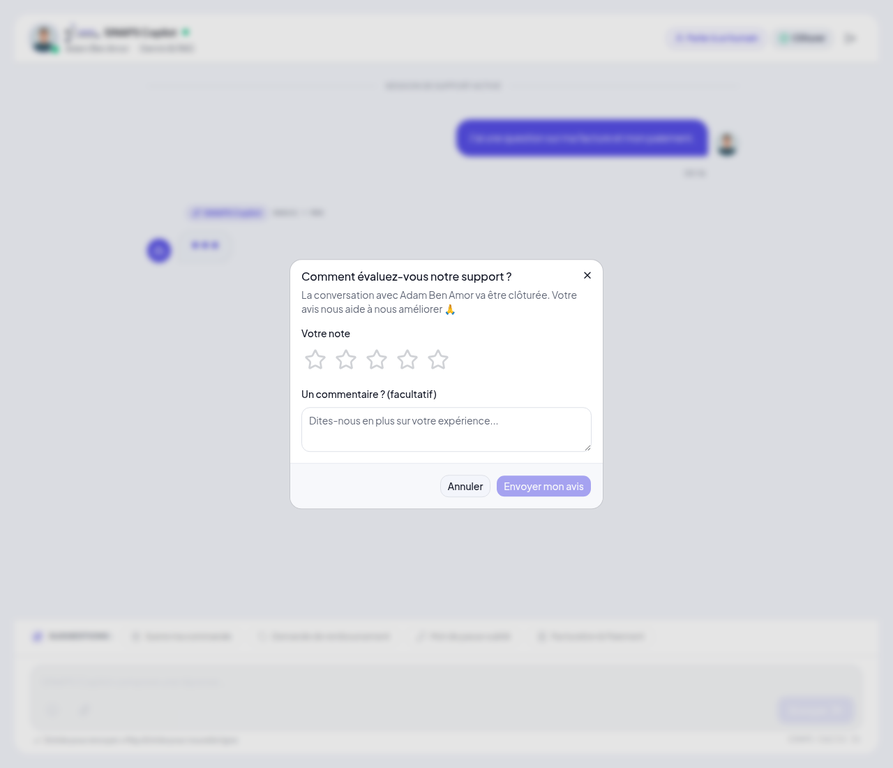
\includegraphics[width=0.9\textwidth]{images/sinaps-satisfaction-dialog.png}
  \caption{Évaluation de la satisfaction à la clôture d'une conversation}
  \label{fig:satisfaction-dialog}
\end{figure}

Les réponses IA peuvent porter des \textbf{actions rapides} : confirmer que la réponse a suffi, poser une autre question ou demander un agent humain. Une action est envoyée comme message client et son état de chargement est affiché ; les boutons ne sont proposés que sur le dernier message IA éligible. Le compositeur est verrouillé pendant la génération IA afin d'éviter les doublons.

\begin{figure}[H]
  \centering
  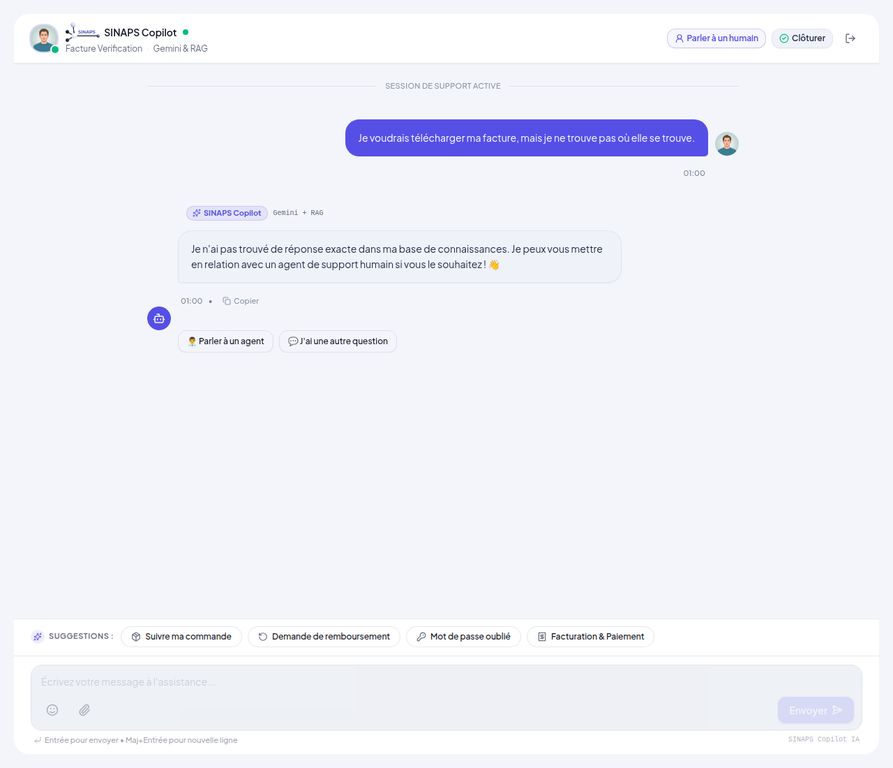
\includegraphics[width=0.9\textwidth]{images/sinaps-client-chat-ai.png}
  \caption{Conversation client avec réponse RAG/Gemini et actions rapides}
  \label{fig:client-chat-ai}
\end{figure}

\subsection{Espace agent}

La page \texttt{/agent} est protégée (\texttt{AuthGuard}). L'agent se connecte sur \texttt{/login}. L'inscription se fait sur \texttt{/agent/signup} (compétences en texte). Tant que le compte est \texttt{pending}, le login renvoie une erreur 403.

\begin{figure}[H]
  \centering
  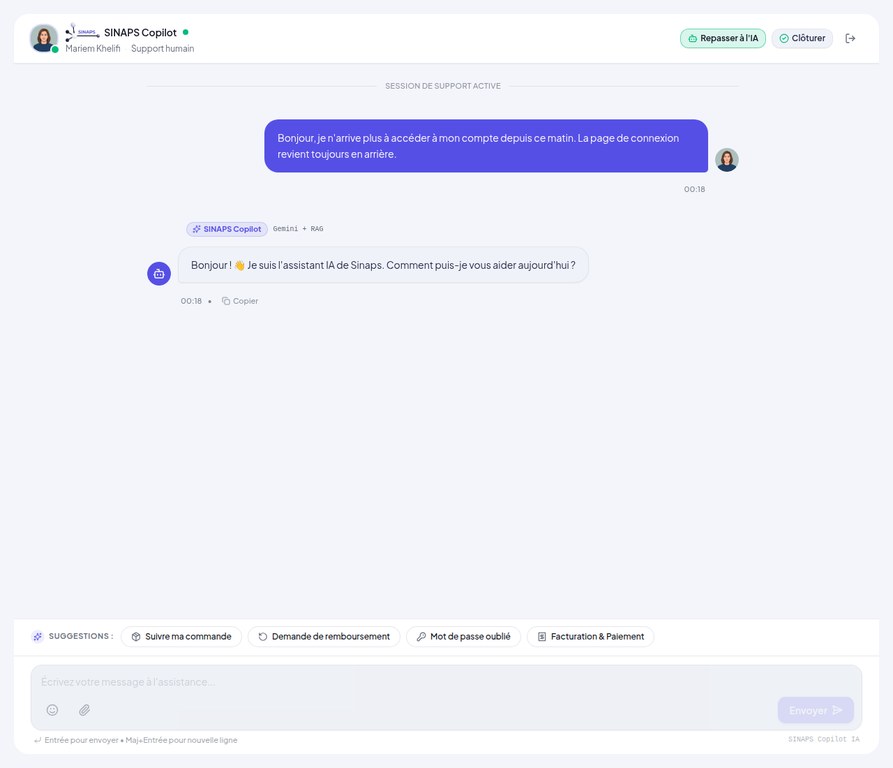
\includegraphics[width=0.9\textwidth]{images/sinaps-human-escalation.png}
  \caption{Escalade d'une conversation vers la file des agents}
  \label{fig:human-escalation}
\end{figure}

\subsection{Espace administrateur}

Le tableau de bord affiche les indicateurs SLA calculés, la liste des agents à valider (compétences en badges), et un historique avec recherche (nom / e-mail client) et onglets de statut. Les conversations marquées comme données de test sont exclues des indicateurs et des listes opérationnelles par défaut. Les dernières corrections ont également stabilisé le chargement concurrent des conversations, le rendu des horodatages et les avatars de repli côté client.

\begin{figure}[H]
  \centering
  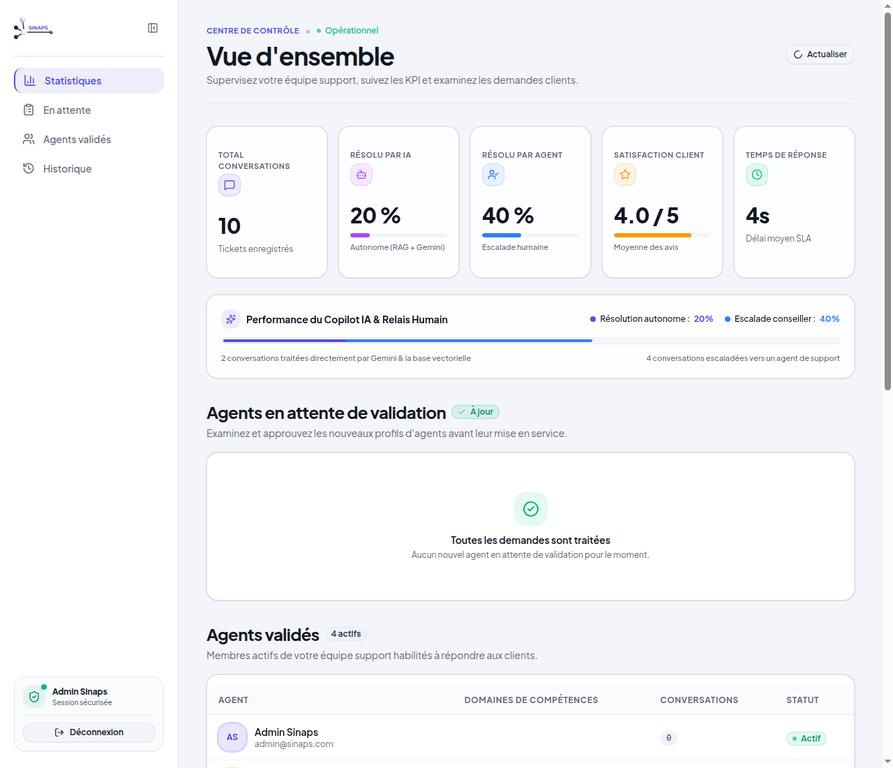
\includegraphics[width=0.95\textwidth]{images/sinaps-admin-dashboard.png}
  \caption{Tableau de bord administrateur de SINAPS TEC}
  \label{fig:admin-dashboard}
\end{figure}

\section{Données de démonstration}

Le script \texttt{npm run seed} recrée des comptes d'exemple (mot de passe de seed : \texttt{password123}) : administrateur \texttt{admin@sinaps.com}, agents validés et un agent en attente, plus des utilisateurs et conversations de démonstration. Ces comptes servent aux captures et aux tests manuels ; ils ne constituent pas une population réelle de production.

\section{Captures d'écran à insérer}

Les captures ci-dessous sont des \textbf{recommandations de documentation}, et non des résultats inventés. Les captures importantes montrent les parcours fonctionnels principaux ; les captures optionnelles peuvent être regroupées ou remplacées par les diagrammes déjà présents au chapitre~3.

\begin{enumerate}[leftmargin=1.6em]
  \item \textbf{Important --- Chat IA et actions rapides}. Capture de \texttt{/} après une question documentée, avec réponse IA, horodatage et boutons « C'est ce qu'il me fallait », « autre question » et « agent ». Placement : après le paragraphe sur l'espace client. Caption : \textit{Conversation client avec réponse RAG/Gemini et actions rapides}. Label : \texttt{fig:client-chat-ai}.
  \item \textbf{Important --- Escalade et espace agent}. Capture de \texttt{/} puis \texttt{/agent} montrant le statut en attente, la file et une réponse humaine. Placement : après le paragraphe sur l'espace agent. Caption : \textit{Escalade d'une conversation vers la file des agents}. Label : \texttt{fig:human-escalation}.
  \item \textbf{Important --- Dashboard administrateur}. Capture de \texttt{/admin} montrant les KPI, la validation des agents et l'historique filtrable. Placement : après le paragraphe sur l'espace administrateur. Caption : \textit{Tableau de bord administrateur de SINAPS TEC}. Label : \texttt{fig:admin-dashboard}.
  \item \textbf{Important --- Clôture et satisfaction}. Capture du dialogue de notation 1--5 avec commentaire facultatif. Placement : après le paragraphe sur la satisfaction. Caption : \textit{Évaluation de la satisfaction à la clôture d'une conversation}. Label : \texttt{fig:satisfaction-dialog}.
  \item \textbf{Optionnel --- Identification client}. Capture de \texttt{/} avant connexion, avec Google Sign-In et formulaire direct. Placement : au début de la sous-section « Espace client ». Caption : \textit{Identification du client par Google ou formulaire}. Label : \texttt{fig:client-auth}.
  \item \textbf{Optionnel --- Pièce jointe et profils}. Capture du fil avec une pièce jointe et les avatars client/agent. Placement : après le paragraphe sur l'espace client. Caption : \textit{Message avec pièce jointe et avatars persistés}. Label : \texttt{fig:message-attachment-avatar}.
  \item \textbf{Optionnel --- Inscription et validation}. Capture de \texttt{/agent/signup} puis de la table des agents en attente. Placement : après le paragraphe sur l'espace administrateur. Caption : \textit{Inscription d'un agent et validation administrative}. Label : \texttt{fig:agent-approval}.
\end{enumerate}

Un \textbf{diagramme de séquence} reste préférable à une capture pour expliquer le flux interne RAG $\rightarrow$ Gemini $\rightarrow$ persistance $\rightarrow$ Socket.io ; la figure~\ref{fig:seq-ia} remplit déjà ce rôle.

\section{Mise en route (développement local)}

\begin{lstlisting}[caption={Démarrage local (d'après le README du projet)},label=lst:run]
# MongoDB Atlas : renseigner MONGO_URI
cd sinaps-backend && npm install && npm run seed && npm run dev
cd sinaps-project && npm install && npm run dev
\end{lstlisting}

Variables nécessaires côté backend : \texttt{PORT}, \texttt{MONGO\_URI}, \texttt{JWT\_SECRET}, \texttt{GEMINI\_API\_KEY}, \texttt{GOOGLE\_CLIENT\_ID} ; côté frontend : \texttt{NEXT\_PUBLIC\_API\_URL}, \texttt{NEXT\_PUBLIC\_GOOGLE\_CLIENT\_ID}. Sans clés Google/Gemini, des modes dégradés existent (identification directe, réponses RAG locales). Le dépôt confirme l'intégration de Google Sign-In, Gemini et MongoDB Atlas, mais ne fournit pas de compte rendu détaillé d'une recette manuelle en conditions réelles.

\chapter{Tests et validation}

Les tests décrits ici sont ceux \textbf{présents dans le dépôt} (\texttt{sinaps-backend/tests}). Aucun pourcentage de couverture, aucun temps de réponse mesuré en production et aucun recettage utilisateur formalisé n'est avancé : ces éléments n'ont pas été fournis comme résultats chiffrés du stage.

\section{Stratégie de test}

La stratégie retenue est essentiellement \textbf{automatisée côté backend} :

\begin{itemize}[leftmargin=1.4em]
  \item tests d'\textbf{intégration} HTTP avec Supertest et une base \textbf{MongoDB en mémoire} ;
  \item tests \textbf{unitaires} du middleware d'authentification (modèle Conversation mocké) ;
  \item tests du \textbf{téléversement} (Multer) ;
  \item tests du \textbf{retriever RAG} et du repli \texttt{getAIResponse} sans clé Gemini.
\end{itemize}

Le frontend Next.js ne contient pas de suite de tests unitaires dédiée dans le dépôt. La validation des écrans a été \textbf{manuelle} (usage réel de Google, Gemini et Atlas). Les résultats détaillés de cette validation manuelle : \acompleter{date, scénarios parcourus, anomalies éventuellement notées}.

Commande :

\begin{lstlisting}[caption={Exécution de la suite backend}]
cd sinaps-backend
npm test
\end{lstlisting}

Les sorties chiffrées de la dernière exécution (nombre de tests, succès, échecs) : \acompleter{coller ici le résumé Jest}.

\section{Tests d'intégration API}

Le fichier \texttt{api.test.js} enchaîne notamment :

\begin{table}[H]
\centering
\caption{Exemples de cas --- \texttt{api.test.js}}
\label{tab:t-api}
\small
\begin{tabularx}{\textwidth}{@{}Xll@{}}
\toprule
Cas & Attendu & \\
\midrule
Création d'utilisateur + jeton client & 200, présence de \texttt{token} & \\
\texttt{find-or-create} conversation sans session & 401 & \\
Création de conversation authentifiée & \texttt{handledBy = ia} & \\
Lecture d'un fil sans session & 401 & \\
Lecture par un autre client & 403 & \\
Lecture par le propriétaire & 200 & \\
Escalade & \texttt{humain}, \texttt{en\_attente} & \\
Désescalade & \texttt{ia}, \texttt{en\_cours} & \\
Clôture avec note 5 & \texttt{resolu}, rating 5 & \\
Clôture avec \texttt{rating: 0} & statut résolu, pas de fausse note & \\
\texttt{sender: humain} sans jeton & 401 & \\
\texttt{sender: humain} avec jeton agent & 201 & \\
\texttt{sender: client} sans jeton & 401 & \\
Client sur une conversation étrangère & 403 & \\
Injection \texttt{sender: ia} depuis l'extérieur & 403 & \\
\bottomrule
\end{tabularx}
\end{table}

\section{Tests du middleware d'authentification}

\texttt{auth-middleware.test.js} vérifie \texttt{requireClientAuth}, \texttt{requireConversationAccess} et \texttt{requireSenderAuth} : absence de header, jeton invalide, rôle inadapté, appartenance de conversation. Ces tests n'ont pas besoin d'une instance Mongo réelle (mock du modèle).

\section{Tests d'upload}

\texttt{upload.test.js} fixe une limite basse (1~Mo) pour rester rapide. Cas couverts : refus sans session (401), refus d'un type non autorisé (400), acceptation JPEG client et PDF agent (200), refus de fichier trop volumineux (413), conservation d'une extension courte alphanumérique pour un sous-type image atypique.

\section{Tests du retriever RAG}

\texttt{rag.test.js} contrôle que :

\begin{itemize}[leftmargin=1.4em]
  \item \og Comment suivre ma commande ? \fg{} ramène l'entrée de suivi ;
  \item une demande de remboursement ramène l'entrée correspondante ;
  \item une requête sans rapport (\texttt{xyz123...}) ne retourne aucun document ;
  \item \texttt{getAIResponse} sans clé Gemini contient la consigne \og Mot de passe oublié \fg{} pour la question de réinitialisation.
\end{itemize}

Ces tests valident le \textbf{retriever local} et le \textbf{repli}. Ils ne mesurent pas la qualité linguistique de Gemini en production.

\section{Limites}

\begin{itemize}[leftmargin=1.4em]
  \item pas de tests E2E navigateur (Playwright, Cypress) dans le dépôt ;
  \item pas de tests de charge Socket.io ;
  \item pas de recette formelle signée par l'encadrant documentée ici : \acompleter{si une démonstration a été faite à M.~Kais, indiquer la date} ;
  \item les indicateurs du dashboard dépendent des données présentes (seed ou usage réel) ; ils ne sont pas des KPI d'un service en production.
\end{itemize}

\chapter*{Conclusion générale}
\addcontentsline{toc}{chapter}{Conclusion générale}

Ce PFA a consisté à concevoir et réaliser \textbf{Op Support IA}, une application web de support client dans laquelle un agent IA s'appuie sur une petite base de connaissances, un opérateur humain peut prendre le relais, et un administrateur pilote comptes, historique et indicateurs.

Le travail a été mené \textbf{seul}, à \textbf{distance}, de façon \textbf{informelle}, du 22~juin au 6~septembre~2026, sur un sujet proposé par \textbf{M.~Kais} (SINAPS). L'application livrée comprend un frontend Next.js, un backend Express, une persistance MongoDB Atlas, une authentification Google et JWT, un moteur RAG lexical couplé à Gemini, des WebSockets, un téléversement de fichiers contrôlé, et une suite de tests backend.

Par rapport au document de sujet, le cœur fonctionnel (chat, RAG, escalade, agents, admin, SLA, contenus riches sous forme de pièces jointes, tests) est en place. En revanche, l'\textbf{application mobile native}, le \textbf{routage par compétences}, le \textbf{RAG vectoriel} et le \textbf{déploiement} d'hébergement public n'ont pas été réalisés --- par choix de périmètre, compte tenu de la durée et du caractère individuel du stage.

Sur le plan pédagogique, la principale difficulté a été l'\textbf{apprentissage simultané} de l'écosystème utilisé : Node.js, Express, React, Next.js, et les notions de RAG. Cette montée en compétence a été nécessaire pour livrer une chaîne fullstack cohérente plutôt qu'un prototype d'interface isolé.

Les perspectives naturelles, si le projet se poursuivait (par exemple dans un PFE), seraient : déployer l'application, remplacer le retriever TF-IDF par des embeddings si la base s'enrichit, affecter les files selon les compétences, durcir l'upload (inspection des octets), et ajouter des tests de bout en bout sur l'UI. Ces pistes ne sont pas des engagements déjà tenus.

Nous remercions à nouveau l'encadrant professionnel et, dès qu'il sera désigné, l'encadrant académique, pour l'accompagnement de ce premier projet de fin d'année d'ingénierie logicielle.


\begin{thebibliography}{99}
\bibitem{express}
Express.js, \textit{Fast, unopinionated, minimalist web framework for Node.js}. Documentation officielle. \url{https://expressjs.com/} (consulté en 2026).

\bibitem{nextjs}
Vercel, \textit{Next.js Documentation}. \url{https://nextjs.org/docs} (consulté en 2026).

\bibitem{mongoose}
Mongoose, \textit{Elegant MongoDB object modeling for Node.js}. \url{https://mongoosejs.com/} (consulté en 2026).

\bibitem{mongodb}
MongoDB, \textit{MongoDB Atlas Documentation}. \url{https://www.mongodb.com/docs/atlas/} (consulté en 2026).

\bibitem{socketio}
Socket.IO, \textit{Documentation}. \url{https://socket.io/docs/} (consulté en 2026).

\bibitem{jwt}
Auth0, \textit{JSON Web Tokens}. \url{https://jwt.io/} (consulté en 2026).

\bibitem{gemini}
Google AI, \textit{Gemini API}. \url{https://ai.google.dev/} (consulté en 2026).

\bibitem{googleauth}
Google Identity, \textit{Authenticate with a backend server}. \url{https://developers.google.com/identity/gsi/web} (consulté en 2026).

\bibitem{jest}
Jest, \textit{Delightful JavaScript Testing}. \url{https://jestjs.io/} (consulté en 2026).

\bibitem{rag}
Lewis, P. et al. \textit{Retrieval-Augmented Generation for Knowledge-Intensive NLP Tasks}. NeurIPS, 2020. (référence conceptuelle du terme RAG ; l'implémentation du PFA est un retriever TF-IDF local, distinct des modèles de l'article.)

\bibitem{sujet}
KAIS (encadrant SINAPS), \textit{Projet Stage -- Op Support IA}. Document de cadrage interne, 2026.

\bibitem{readme}
Chaabene, M., \textit{Documentation technique et utilisateur -- Projet Op Support IA (Sinaps)}, fichier \texttt{sinaps-project/README.md} du dépôt, 2026.

\end{thebibliography}

\appendix
\chapter{Annexes}

\section{Glossaire des statuts de conversation}

\begin{table}[H]
\centering
\caption{Statuts et modes de prise en charge}
\label{tab:annexe-statuts}
\begin{tabularx}{\textwidth}{|l|l|X|}
\hline
Champ & Valeur & Signification opérationnelle \\
\hline
status & \texttt{en\_cours} & Conversation active (IA ou humain déjà en charge) \\
\hline
status & \texttt{en\_attente} & Escaladée, en file côté agents \\
\hline
status & \texttt{resolu} & Clôturée \\
\hline
handledBy & \texttt{ia} & Prochaine réponse automatique possible \\
\hline
handledBy & \texttt{humain} & Réponses attendues d'un opérateur \\
\hline
\end{tabularx}
\end{table}

\section{Exemple d'entrée de la base de connaissances}

Les extraits suivants sont des \textbf{exemples} utilisés par le retriever, et non une documentation officielle de produits SINAPS TEC.

\Needspace{9\baselineskip}
\begin{lstlisting}[caption={Extrait de \texttt{knowledgeBase.js}}]
{
  question: "Comment suivre ma commande ?",
  answer: "Vous pouvez suivre votre commande depuis votre espace
           client, section 'Mes commandes'. Un numéro de suivi
           est envoyé par email dès l'expédition."
}
\end{lstlisting}

\section{Comptes du script de seed (environnement de démo)}

Ces identifiants figurent dans le README du projet à des fins de démonstration locale. Ils ne doivent pas être réutilisés en production.

\begin{table}[H]
\centering
\caption{Comptes créés par \texttt{npm run seed}}
\label{tab:seed}
\begin{tabularx}{\textwidth}{|l|l|l|X|}
\hline
Rôle & E-mail & Mot de passe (seed) & Accès \\
\hline
Admin & admin@sinaps.com & password123 & \texttt{/admin} \\
\hline
Agent & sarah.benali@sinaps.com & password123 & \texttt{/agent} \\
\hline
Agent & karim.mansouri@sinaps.com & password123 & \texttt{/agent} \\
\hline
Pending & youssef.mehdi@sinaps.com & password123 & login refusé tant que non validé \\
\hline
\end{tabularx}
\end{table}


\end{document}
